\chapter{Simulated Scenarios}
\label{chap:simulated_scenarios}
This chapter is dedicated to the description of the various simulated scenarios that were tested using the ToD simulation framework, after a brief introduction on the chosen map from CARLA.
They are divided into two sections, as their nature is twofold: one that involves the Host Vehicle completing a trip over a predetermined route with varying levels and types of network background, and one that tests the feasibility of the reaction to obstacles by the ToD operator and how it is influenced by growing levels of background traffic.

\section{Simulation map}
The chosen map from CARLA used in all simulations is \texttt{Town04}, shown in \figurename~\ref{fig:carla_town04_aerial}, which consists of a small town rounded by a multi-lane highway laid in a ``figure of 8'' shape, which intersects with itself in the center of the map in a cloverleaf interchange~\cite{carladoc}.

\begin{figure}[h]
    \centering
    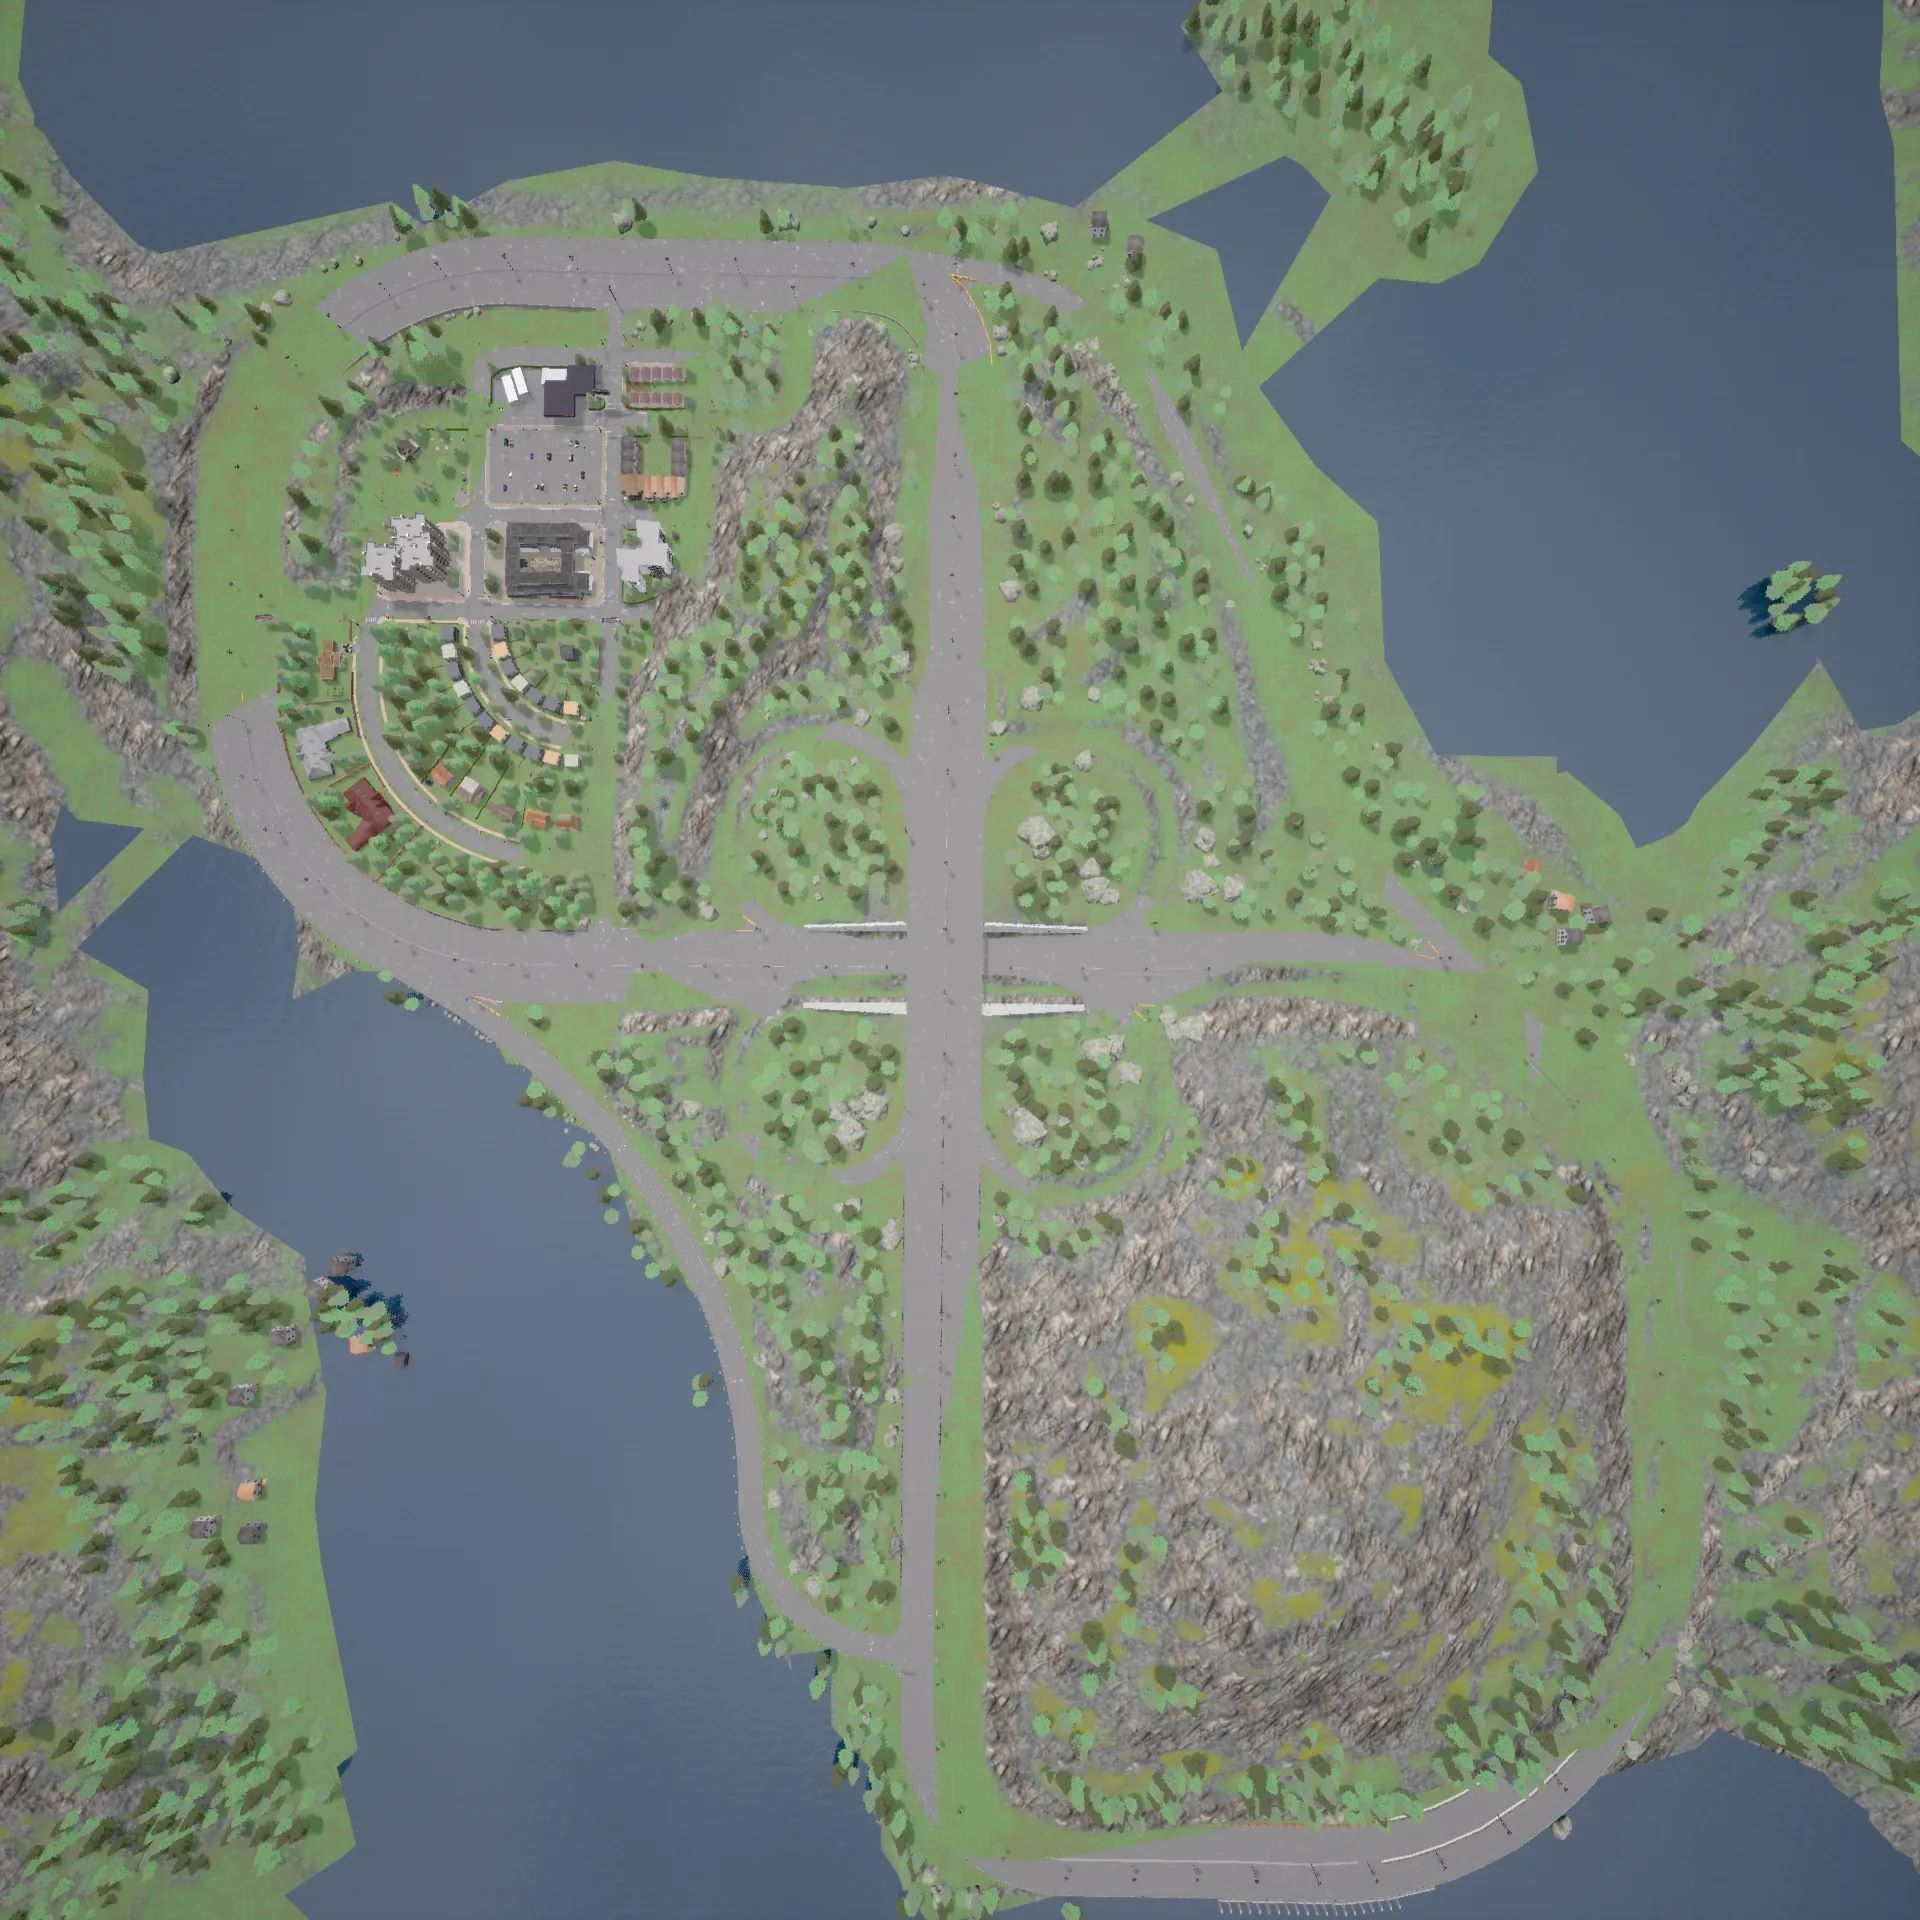
\includegraphics[width=.7\textwidth]{scenarios/carla_town04_aerial}
    \caption{Aerial view of CARLA map Town04, from \cite{carladoc}}
    \label{fig:carla_town04_aerial}
\end{figure}

%\section{Scenarios description}
\section{City trip}
%\label{sec:scenarios:city_trip}
This scenario takes the route specified in \cite{valeriopaper} and tests it against varying network configurations and loads.

The selected route goes as follows: It starts on the north section of the ``ring road'' going south, takes a slip road heading south-west with a speed limit of 60km/h for the first smooth curve, crosses a junction with a 30 and then 40km/h limit into the highway again heading east at 90km/h towards the center of the map. Once there, the speed limit decreases to 60km/h and then 30km/h into the slip road going north. Then, after a short 90km/h stretch of highway it turns right into the city where the final 30km/h section begins. Once there it makes a left and leads into the center of the city where the end waypoint is. A drawing of the route on the map color-coded with the different speed limits is visible in \figurename~\ref{fig:valerios_sim_trajectory_route}.

\begin{figure}[h]
    \centering
    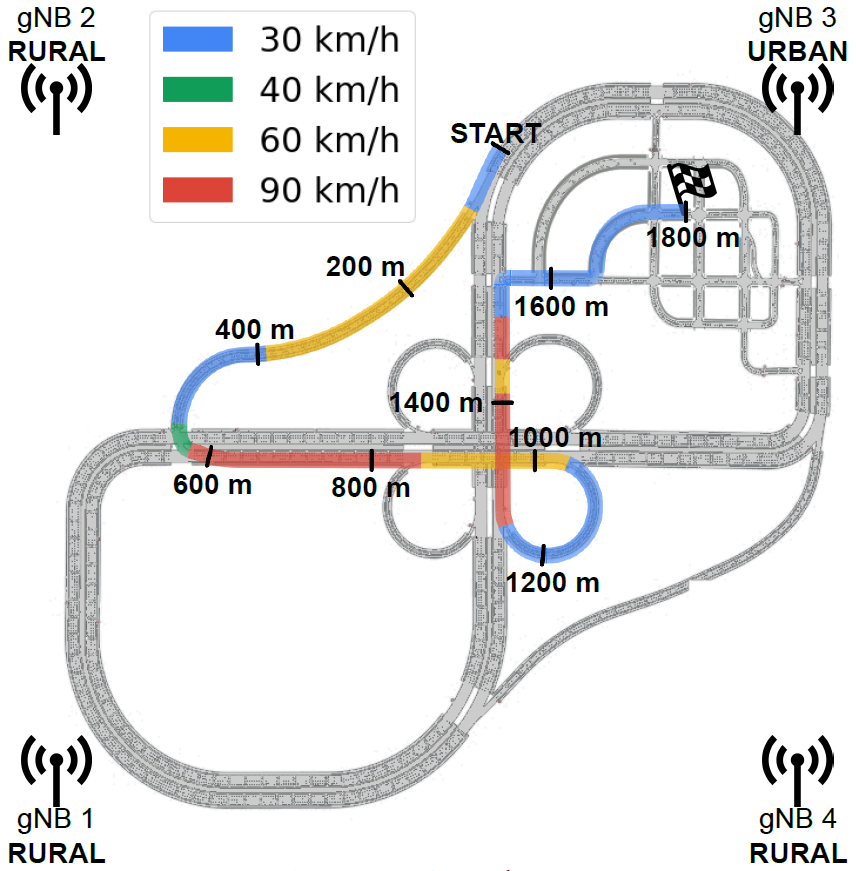
\includegraphics[width=.8\textwidth]{valeriopaper/trajectory_route}
    \caption{City trip route to follow overlaid on the road map of Town04 showing speed limits, from \cite{valeriopaper}}
    \label{fig:valerios_sim_trajectory_route}
\end{figure}

\subsection{Background}
\label{subsec:scenarios:city_trip:background}
The base scenario takes into consideration the presence of a single user on the network, which is far from a realistic simulation, so a way to generate some background traffic was needed.
The background was simulated in two different ways:
\subsubsection{Static background}
This takes the same form as the simulations described in \cite{valeriopaper}, where up to three nodes are spawned in the OMNeT++ simulation around each base station and they produce a comparable amount of traffic as the same number of other HVs running a ToD service.

\subsubsection{Moving background}
The static background simulation works and it will be shown that it does have an influence over the feasibility of certain parameter configurations, but it does so in a pretty linear and predictable fashion. The following introduces a different perspective on background generation: instead of keeping the same number of background users in fixed positions around each base station, up to three CARLA actors are roaming around the same area as the Host Vehicle, to better simulate scenarios where other users are on the road and putting varying load on the base stations, influenced by their distance from the base station and channel quality, making their impact on the overall service less predictable.

In order to keep consistency on the route across simulations, the background vehicle routes are set up so that they will not interfere with the HV by making it slow down or stop.


\section{Reaction to obstacles}
This section describes the different simulated scenarios that involve the presence of an obstacle on the HV's path prompting a reaction by the ToD operator, both present from the start and suddenly appearing in an urban environment, and suddenly appearing in a highway or extra-urban environment.

\subsection{Static obstacle}
\label{subsec:scenarios:city_static_obstacle}

\begin{figure}[h]
    \centering
    \includegraphics[width=\textwidth]{scenarios/city_static_obstacle/render_safe/montage}
    \caption{City static obstacle scenario rendered by CARLA}
    \label{fig:scenarios_static_obs_safe}
\end{figure}
In this scenario, an obstacle is placed on the vehicle's path from the start of the simulation (\figurename~\ref{fig:scenarios_static_obs_safe}). The route is very short as is the overall duration of simulations. The vehicle reaches a speed of 30km/h and then has to brake in order to avoid a collision.

\subsection{City sudden obstacle}
The nature of this scenario is the same as Section~\ref{subsec:scenarios:city_static_obstacle} except the obstacle only appears in the world when the Host Vehicle is 10m away from the obstacle's spawn point (\figurename~\ref{fig:scenarios_sudden_obs_safe_crash}). This is a scenario similar to a distracted pedestrian or a pet suddenly crossing the street without looking.

\begin{figure}[h]
    \centering
    \begin{subfigure}[b]{\textwidth}
        \centering
        \includegraphics[width=\textwidth]{scenarios/city_sudden_obstacle/render_safe/montage}
        \caption{No crash}
    \end{subfigure}
    \hfill
    \begin{subfigure}[b]{\textwidth}
        \centering
        \includegraphics[width=\textwidth]{scenarios/city_sudden_obstacle/render_crash/montage}
        \caption{Crash}
    \end{subfigure}
    \caption{City sudden obstacle scenario rendered by CARLA}
    \label{fig:scenarios_sudden_obs_safe_crash}
\end{figure}


\subsection{Highway sudden obstacle}
This scenario follows the purpose of evaluating the feasibility of the reaction by the ToD operator to an obstacle suddenly appearing on the Host Vehicle's path. The event takes place on a highway section, where the obstacle appears in the world when the HV is 44m away from its spawn point and traveling at a speed of 90km/h.


\section{Simulation Parameters}
The complex nature of the simulators, particularly OMNeT++, offers immense parameter customization down to the most specific details. Table~\ref{tab:simulation_parameters} contains a relevant subset of parameters that make up the overall configuration and this section will explain the most relevant ones considered when defining the parameter study.

\subsection{Number of background users}
This parameter regulates how many background users are simulated around each base station as the static background and how many users are roaming the streets as the moving background. The latter is only used in some of the tested city trip scenarios. All other cases use the static background.
For the purpose of this thesis between 0 and 3 of them will be considered.

\subsection{Numerology}

Numerology in the context of 5G NR (New Radio) defines the chosen subcarrier spacing ($\Delta f$) as per the following formula \cite{ETSITS138300}:

$$\Delta f=2^\mu \times 15\text{kHz}$$ 

Subcarrier Spacing ($\Delta f$) determines the frequency granularity of the system. Smaller subcarrier spacings provide higher frequency resolution but may result in larger symbol durations. Conversely, larger subcarrier spacings offer better spectral efficiency but with coarser frequency resolution.
For our data transmissions, we will only consider $\mu$ values of 0 and 1, i.e.\ 15 and 30 kHz.

The symbol duration is inversely proportional to the subcarrier spacing. Transmissions are organized in time slots, each of those containing 14 symbols. For numerology 0, a time slot lasts 1ms, while for numerology 1 it's half that: 0.5ms, because of the wider subcarrier spacing. More specifically, the symbol duration is 66.7µs for a numerology index of 0 and 33.3µs for a numerology index of 1. It will be shown that this helps greatly with overall latency.

\subsection{Packet size \& Frame rate}
These two parameters are tightly related as together they make up the effective bitrate of the data transmissions.
The packet size refers to the size in kilobytes of each status packet sent by the Host Vehicle to the ToD operator through the network.
The frame rate, expressed in frames per second or fps, defines how many times per second this transmission is made.

A bigger packet size represents a higher quality video stream and a higher frame rate allows the operator to respond to information that is more up-to-date thanks to the higher sampling frequency.
The overall bitrate can be calculated using the formula:

$$\text{bitrate (Mbps)} = \frac{\text{status packet size (kB)}}{1024} * 8 * \text{frame rate}$$

The least demanding and lowest quality configuration is the one with 33kB packet size (HD video) and a frame rate of 25fps, which amounts to around 6.5Mbps, while the most demanding and higher quality configuration is the one with 66kB packet size (Full HD video) and a frame rate of 60fps, which amounts to around 31Mbps.

\subsection{Number of resource blocks}

A resource block consists of 12 consecutive subcarriers, and while the work presented in \cite{valeriopaper} uses a fixed number of resource blocks for both numerology values, this thesis will employ 100 of them for $\mu=0$ and 50 for $\mu=1$, so that the available bandwidth stays constant across all simulations (20MHz). It will be shown in Chapter~\ref{chap:results} that this brings a change with respect to the original scenarios in more demanding configurations.


\begingroup
\renewcommand{\arraystretch}{1}
\begin{table}[t]
\begin{center}
%\footnotesize
 \begin{tabular*}{.8\textwidth}{l@{\extracolsep{\fill}}r}
 \hline 
 \large	\textbf{Parameter} & \large	\textbf{Value} \\ 
 \hline 
 \hline
 \multirow{1}{*}{\textbf{Numerology index ($\mu$)}}
 & \textit{0, 1} \\
 \hline
 \multirow{2}{*}{\textbf{Frame rate}}
 & \textit{25~fps} \\
 & \textit{60~fps} \\
 \hline
 \multirow{2}{*}{\textbf{Status packet size}}
 & \textit{33~kB} \\
 & \textit{66~kB} \\
 \hline
 \multirow{1}{*}{\textbf{Instruction packet size}}
 & \textit{1000~B} \\
 \hline
 \multirow{1}{*}{\textbf{Encoding image time}}
 & \textit{normal(10~ms, 0.5~ms)} \\
 \hline
 \multirow{1}{*}{\textbf{Collection data time}}
 & \textit{normal(15ms, 0.1ms)} \\
 \hline
 \multirow{1}{*}{\textbf{Processing status time}}
 & \textit{normal(15ms, 0.75ms)}  \\
 \hline
 \multirow{1}{*}{\textbf{gNodeB mac scheduler}}
 & \textit{Round-robin}  \\
 \hline
 \multirow{1}{*}{\textbf{Handover latency}}
 & \textit{50~ms}  \\
 \hline
 \multirow{1}{*}{\textbf{Target BLER}}
 & \textit{0.01}  \\
 \hline
 \multirow{1}{*}{\textbf{Resource blocks}}
 & \textit{100} if $\mu=0$, \textit{50} if $\mu=1$  \\
 \hline
 \multirow{1}{*}{\textbf{ToD background cars count}}
 & \textit{0, 1, 2, 3}\\
 \hline
 \multirow{1}{*}{\textbf{Background status packet size}}
 & \textit{33~kB}\\
 \hline
 \multirow{2}{*}{\textbf{\shortstack[l]{ToD driving simulation\\time-step}}}
 & \textit{10~ms}\\
 & \\
 \hline
\end{tabular*}
\caption{Simulation parameters used}
\label{tab:simulation_parameters}
\end{center}
\end{table}
\endgroup
